\documentclass[11pt]{article}
\usepackage[textwidth=18.0cm, textheight=23.0cm, top=2.0cm]{geometry}
\usepackage{pst-all}
\usepackage{amssymb}
\usepackage{tikz}
\usepackage{underscore}\begin{document}
\pagestyle{empty}


ClassName: \underline{\textbf{Class_10.2bp-32}}
\par
BinSize: \underline{\textbf{100 × 100}}
\par
ReduceSize: \underline{\textbf{100 × 100}}
\par
TypeNum: \underline{\textbf{80}}
\par
Num: \underline{\textbf{80}}
\par
OutS: \underline{\textbf{110000}}
\par
InS: \underline{\textbf{101043}}
\par
Rate: \underline{\textbf{0.919}}
\par
UB: \underline{\textbf{11}}
\par
LB0: \underline{\textbf{11}}
\par
LB: \underline{\textbf{11}}
\par
LBWithCut: \underline{\textbf{11}}
\par
NodeCut: \underline{\textbf{0}}
\par
ExtendedNodeCnt: \underline{\textbf{1}}
\par
GenNodeCnt: \underline{\textbf{1}}
\par
PrimalNode: \underline{\textbf{0}}
\par
ColumnCount: \underline{\textbf{11}}
\par
TotalCutCount: \underline{\textbf{0}}
\par
RootCutCount: \underline{\textbf{0}}
\par
LPSolverCnt: \underline{\textbf{1}}
\par
PricingSolverCnt: \underline{\textbf{0}}
\par
BranchAndBoundNum: \underline{\textbf{1}}
\par
isOpt: \underline{\textbf{true}}
\par
TimeOnInitSolution: \underline{\textbf{600.000 s}}
\par
TimeOnPrimal: \underline{\textbf{0.000 s}}
\par
TimeOnPricing: \underline{\textbf{0.000 s}}
\par
TimeOnRmp: \underline{\textbf{0.078 s}}
\par
TotalTime: \underline{\textbf{600.360 s}}
\par
\newpage


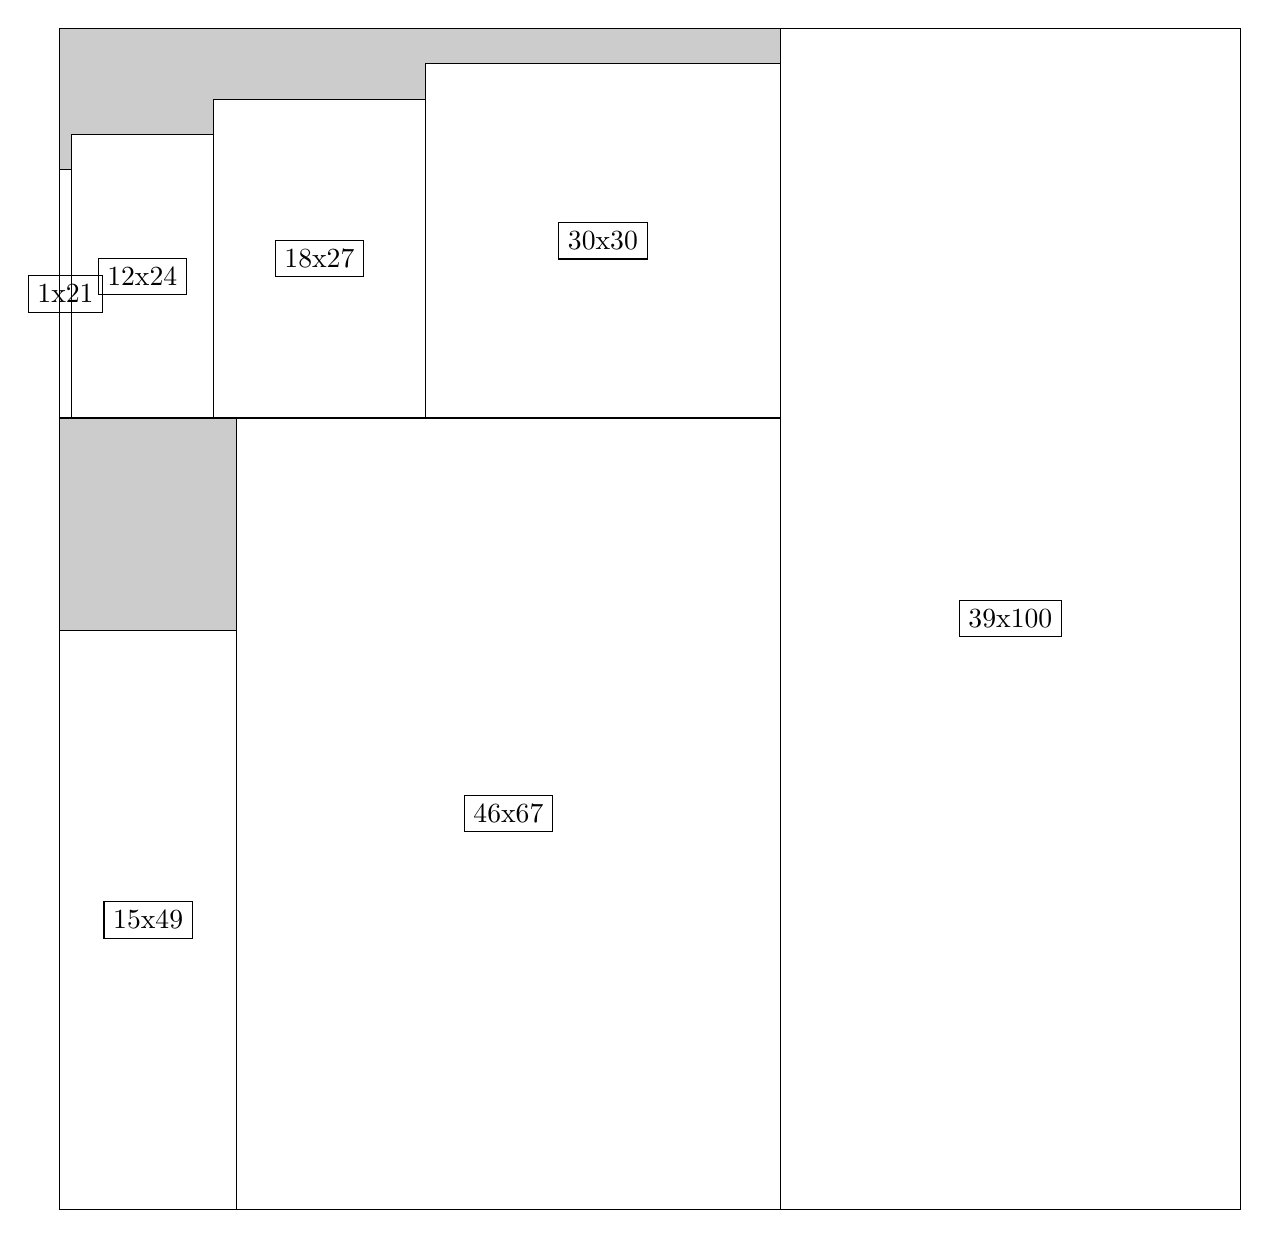
\begin{tikzpicture}[shorten >=1pt,scale=1.0,every node/.style={scale=1.0},->]
\tikzstyle{vertex}=[circle,fill=black!25,minimum size=14pt,inner sep=0pt]
\filldraw[fill=gray!40!white, draw=black] (0,0) rectangle (15.0,15.0);
\foreach \name/\x/\y/\w/\h in {39x100/9.15/0.0/5.85/15.0,46x67/2.25/0.0/6.8999999999999995/10.049999999999999,15x49/0.0/0.0/2.25/7.35,30x30/4.6499999999999995/10.049999999999999/4.5/4.5,18x27/1.95/10.049999999999999/2.6999999999999997/4.05,12x24/0.15/10.049999999999999/1.7999999999999998/3.5999999999999996,1x21/0.0/10.049999999999999/0.15/3.15}
\filldraw[fill=white!40!white, draw=black] (\x,\y) rectangle node[draw] (\name) {\name} ++(\w,\h);
\end{tikzpicture}


w =39 , h =100 , x =61 , y =0 , v =3900
\par
w =46 , h =67 , x =15 , y =0 , v =3082
\par
w =15 , h =49 , x =0 , y =0 , v =735
\par
w =30 , h =30 , x =31 , y =67 , v =900
\par
w =18 , h =27 , x =13 , y =67 , v =486
\par
w =12 , h =24 , x =1 , y =67 , v =288
\par
w =1 , h =21 , x =0 , y =67 , v =21
\par
\newpage


\begin{tikzpicture}[shorten >=1pt,scale=1.0,every node/.style={scale=1.0},->]
\tikzstyle{vertex}=[circle,fill=black!25,minimum size=14pt,inner sep=0pt]
\filldraw[fill=gray!40!white, draw=black] (0,0) rectangle (15.0,15.0);
\foreach \name/\x/\y/\w/\h in {99x78/0.15/0.0/14.85/11.7,1x41/0.0/0.0/0.15/6.1499999999999995,93x21/1.05/11.7/13.95/3.15,7x11/0.0/11.7/1.05/1.65,96x1/0.6/14.85/14.399999999999999/0.15}
\filldraw[fill=white!40!white, draw=black] (\x,\y) rectangle node[draw] (\name) {\name} ++(\w,\h);
\end{tikzpicture}


w =99 , h =78 , x =1 , y =0 , v =7722
\par
w =1 , h =41 , x =0 , y =0 , v =41
\par
w =93 , h =21 , x =7 , y =78 , v =1953
\par
w =7 , h =11 , x =0 , y =78 , v =77
\par
w =96 , h =1 , x =4 , y =99 , v =96
\par
\newpage


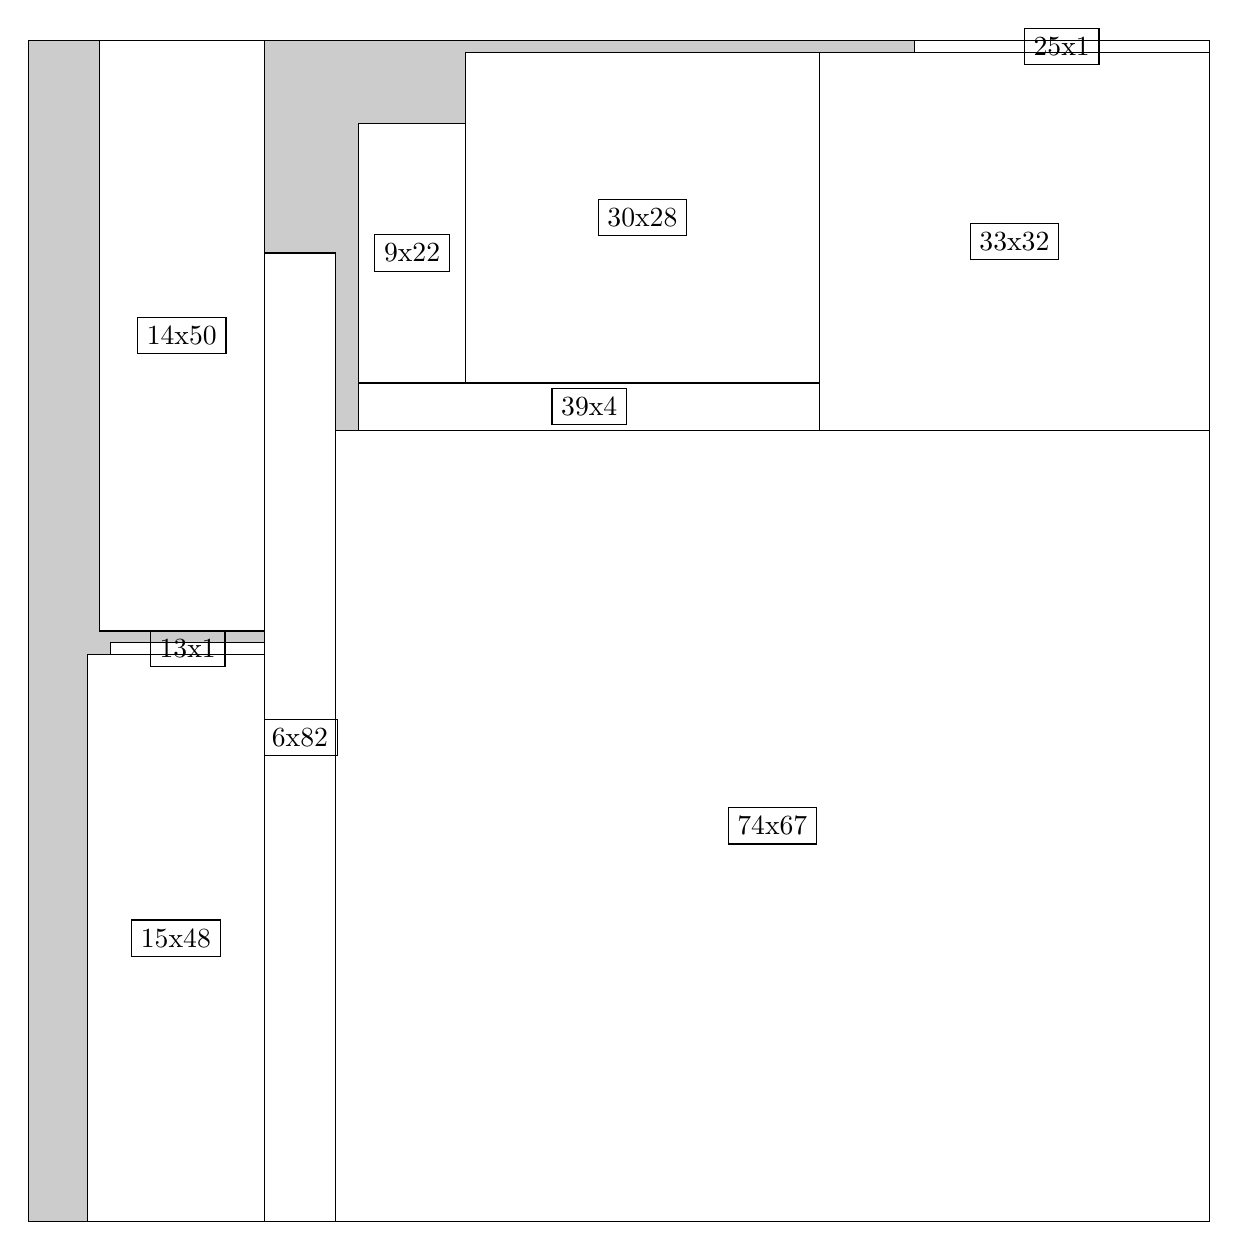
\begin{tikzpicture}[shorten >=1pt,scale=1.0,every node/.style={scale=1.0},->]
\tikzstyle{vertex}=[circle,fill=black!25,minimum size=14pt,inner sep=0pt]
\filldraw[fill=gray!40!white, draw=black] (0,0) rectangle (15.0,15.0);
\foreach \name/\x/\y/\w/\h in {74x67/3.9/0.0/11.1/10.049999999999999,33x32/10.049999999999999/10.049999999999999/4.95/4.8,25x1/11.25/14.85/3.75/0.15,39x4/4.2/10.049999999999999/5.85/0.6,30x28/5.55/10.65/4.5/4.2,9x22/4.2/10.65/1.3499999999999999/3.3,6x82/3.0/0.0/0.8999999999999999/12.299999999999999,15x48/0.75/0.0/2.25/7.199999999999999,13x1/1.05/7.199999999999999/1.95/0.15,14x50/0.8999999999999999/7.5/2.1/7.5}
\filldraw[fill=white!40!white, draw=black] (\x,\y) rectangle node[draw] (\name) {\name} ++(\w,\h);
\end{tikzpicture}


w =74 , h =67 , x =26 , y =0 , v =4958
\par
w =33 , h =32 , x =67 , y =67 , v =1056
\par
w =25 , h =1 , x =75 , y =99 , v =25
\par
w =39 , h =4 , x =28 , y =67 , v =156
\par
w =30 , h =28 , x =37 , y =71 , v =840
\par
w =9 , h =22 , x =28 , y =71 , v =198
\par
w =6 , h =82 , x =20 , y =0 , v =492
\par
w =15 , h =48 , x =5 , y =0 , v =720
\par
w =13 , h =1 , x =7 , y =48 , v =13
\par
w =14 , h =50 , x =6 , y =50 , v =700
\par
\newpage


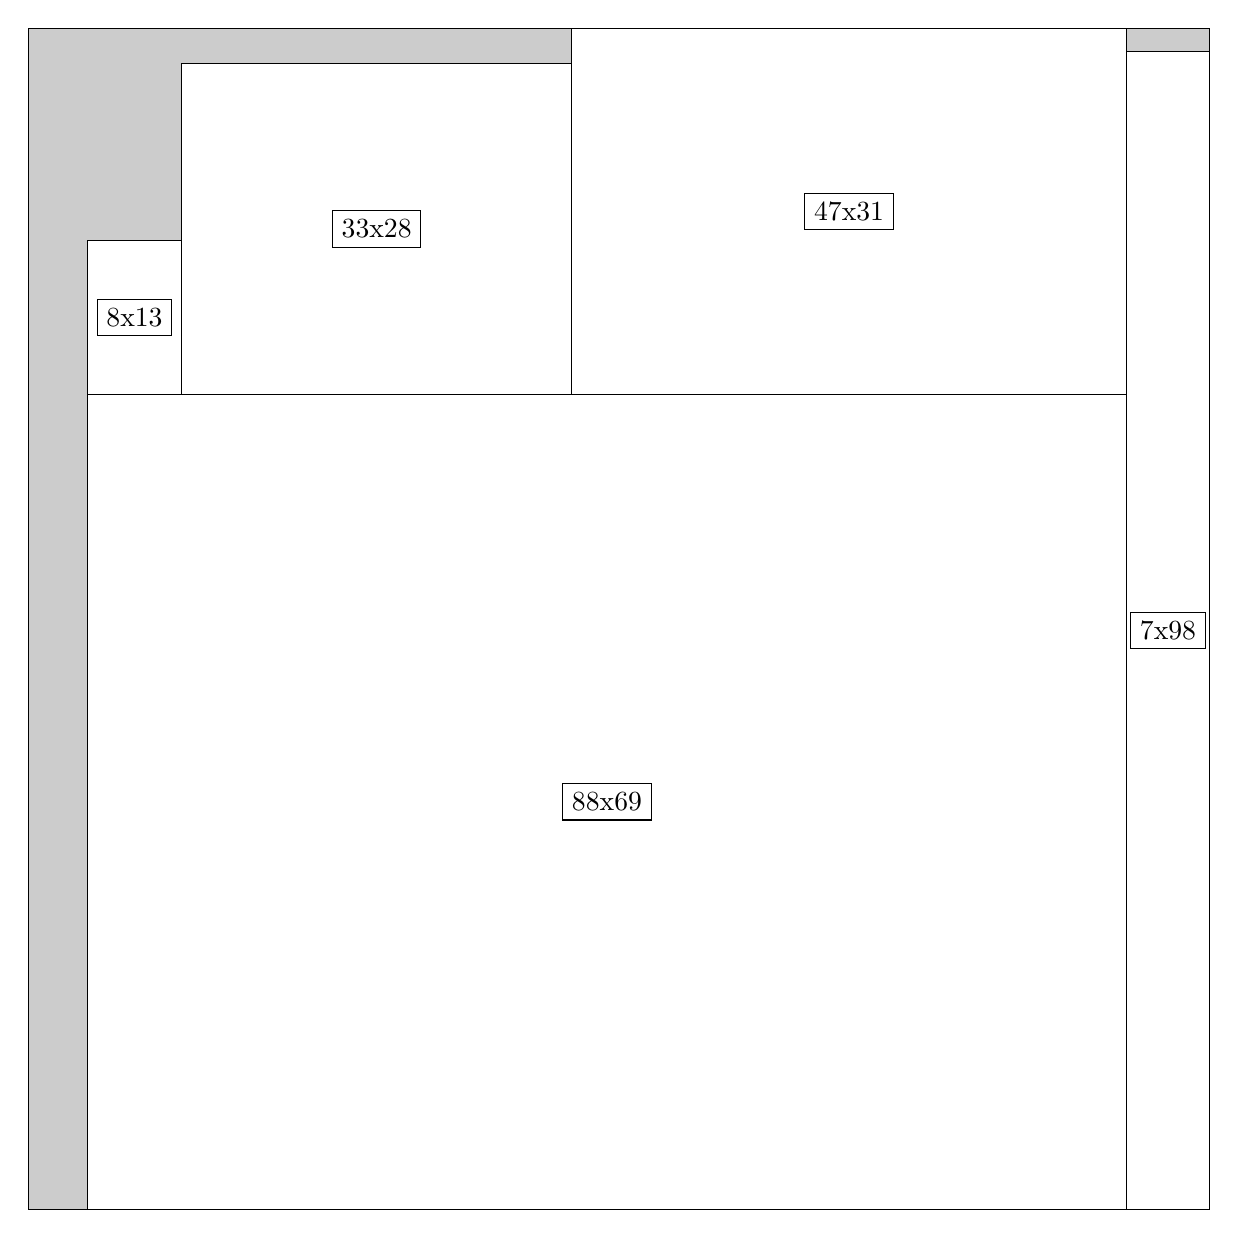
\begin{tikzpicture}[shorten >=1pt,scale=1.0,every node/.style={scale=1.0},->]
\tikzstyle{vertex}=[circle,fill=black!25,minimum size=14pt,inner sep=0pt]
\filldraw[fill=gray!40!white, draw=black] (0,0) rectangle (15.0,15.0);
\foreach \name/\x/\y/\w/\h in {7x98/13.95/0.0/1.05/14.7,88x69/0.75/0.0/13.2/10.35,47x31/6.8999999999999995/10.35/7.05/4.6499999999999995,33x28/1.95/10.35/4.95/4.2,8x13/0.75/10.35/1.2/1.95}
\filldraw[fill=white!40!white, draw=black] (\x,\y) rectangle node[draw] (\name) {\name} ++(\w,\h);
\end{tikzpicture}


w =7 , h =98 , x =93 , y =0 , v =686
\par
w =88 , h =69 , x =5 , y =0 , v =6072
\par
w =47 , h =31 , x =46 , y =69 , v =1457
\par
w =33 , h =28 , x =13 , y =69 , v =924
\par
w =8 , h =13 , x =5 , y =69 , v =104
\par
\newpage


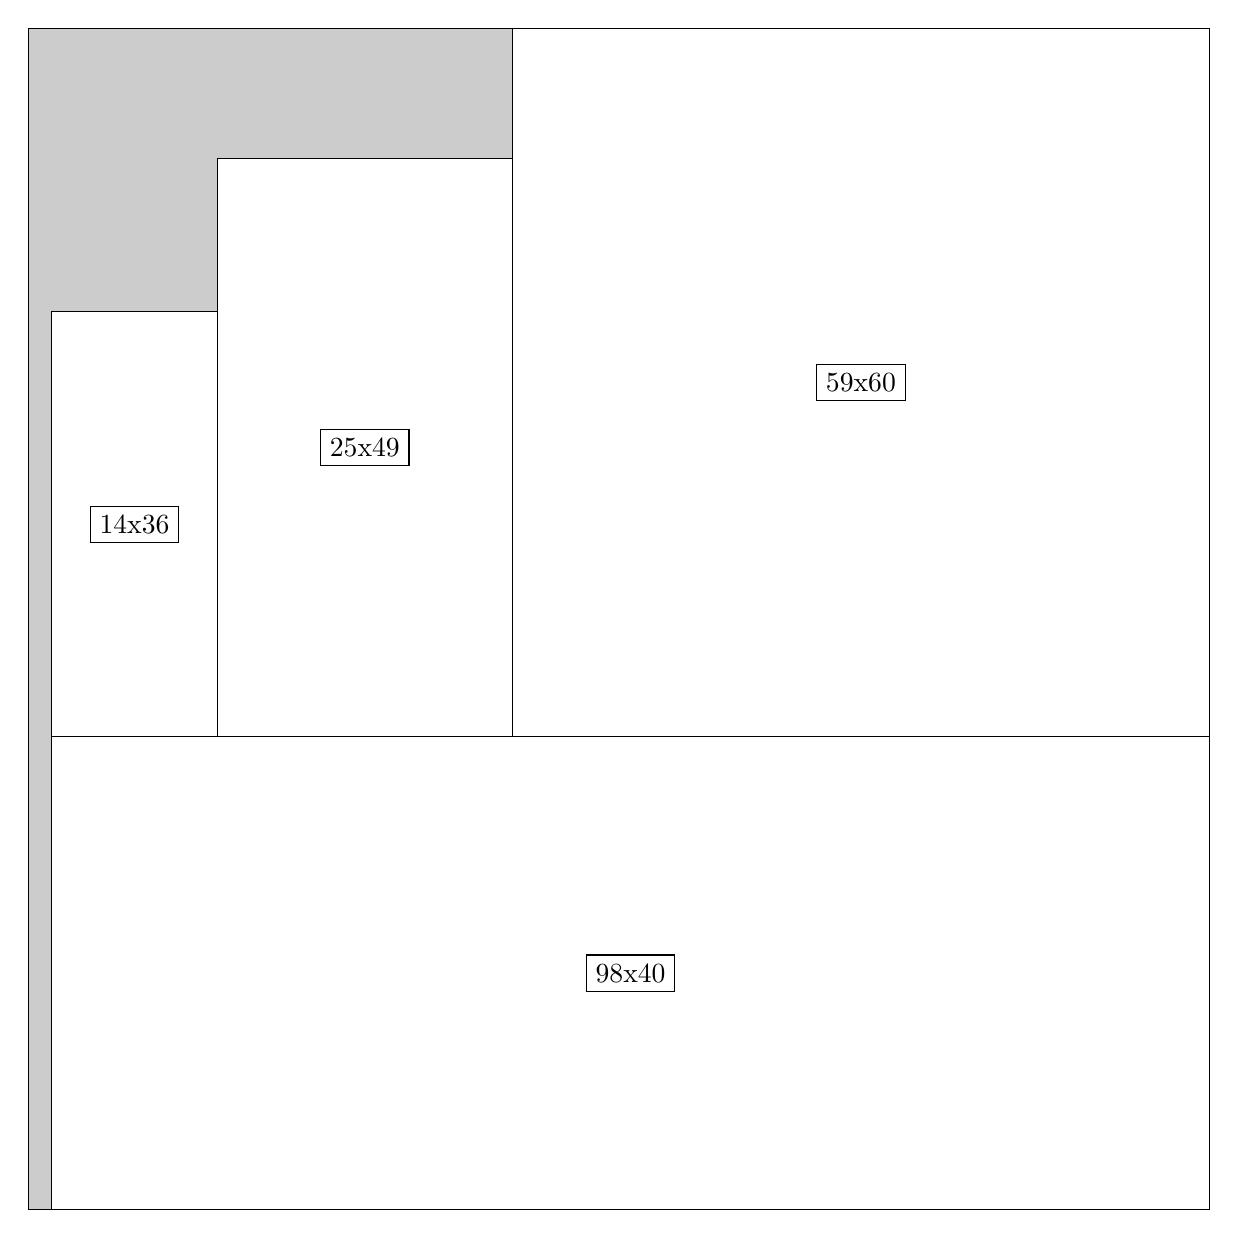
\begin{tikzpicture}[shorten >=1pt,scale=1.0,every node/.style={scale=1.0},->]
\tikzstyle{vertex}=[circle,fill=black!25,minimum size=14pt,inner sep=0pt]
\filldraw[fill=gray!40!white, draw=black] (0,0) rectangle (15.0,15.0);
\foreach \name/\x/\y/\w/\h in {98x40/0.3/0.0/14.7/6.0,59x60/6.1499999999999995/6.0/8.85/9.0,25x49/2.4/6.0/3.75/7.35,14x36/0.3/6.0/2.1/5.3999999999999995}
\filldraw[fill=white!40!white, draw=black] (\x,\y) rectangle node[draw] (\name) {\name} ++(\w,\h);
\end{tikzpicture}


w =98 , h =40 , x =2 , y =0 , v =3920
\par
w =59 , h =60 , x =41 , y =40 , v =3540
\par
w =25 , h =49 , x =16 , y =40 , v =1225
\par
w =14 , h =36 , x =2 , y =40 , v =504
\par
\newpage


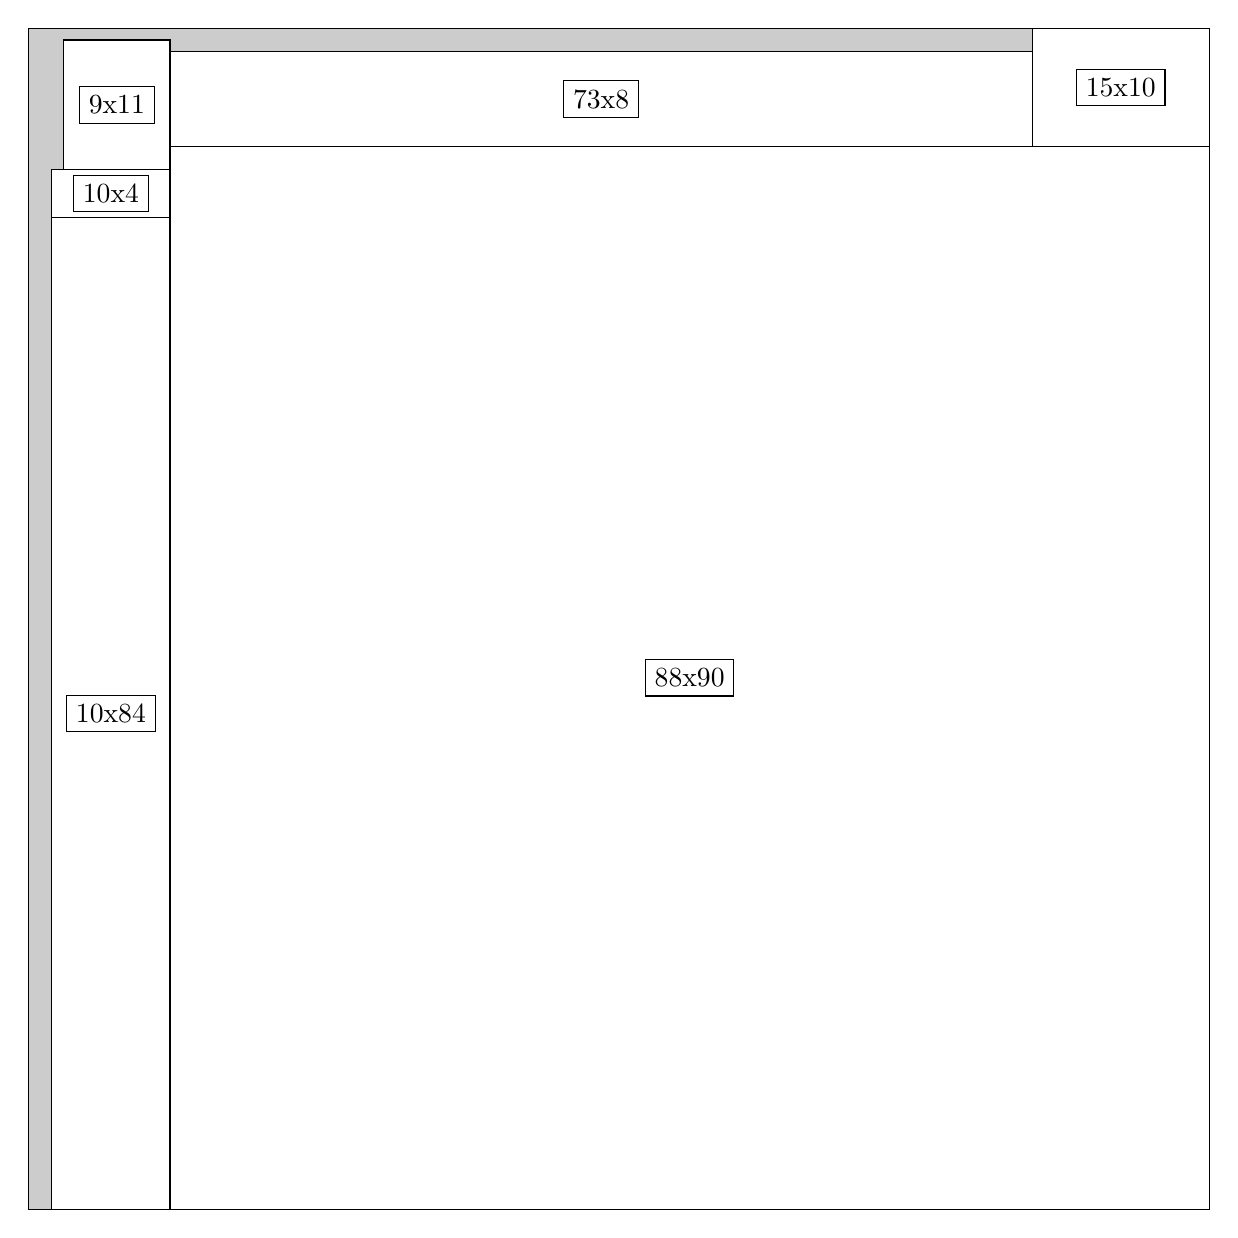
\begin{tikzpicture}[shorten >=1pt,scale=1.0,every node/.style={scale=1.0},->]
\tikzstyle{vertex}=[circle,fill=black!25,minimum size=14pt,inner sep=0pt]
\filldraw[fill=gray!40!white, draw=black] (0,0) rectangle (15.0,15.0);
\foreach \name/\x/\y/\w/\h in {88x90/1.7999999999999998/0.0/13.2/13.5,15x10/12.75/13.5/2.25/1.5,73x8/1.7999999999999998/13.5/10.95/1.2,10x84/0.3/0.0/1.5/12.6,10x4/0.3/12.6/1.5/0.6,9x11/0.44999999999999996/13.2/1.3499999999999999/1.65}
\filldraw[fill=white!40!white, draw=black] (\x,\y) rectangle node[draw] (\name) {\name} ++(\w,\h);
\end{tikzpicture}


w =88 , h =90 , x =12 , y =0 , v =7920
\par
w =15 , h =10 , x =85 , y =90 , v =150
\par
w =73 , h =8 , x =12 , y =90 , v =584
\par
w =10 , h =84 , x =2 , y =0 , v =840
\par
w =10 , h =4 , x =2 , y =84 , v =40
\par
w =9 , h =11 , x =3 , y =88 , v =99
\par
\newpage


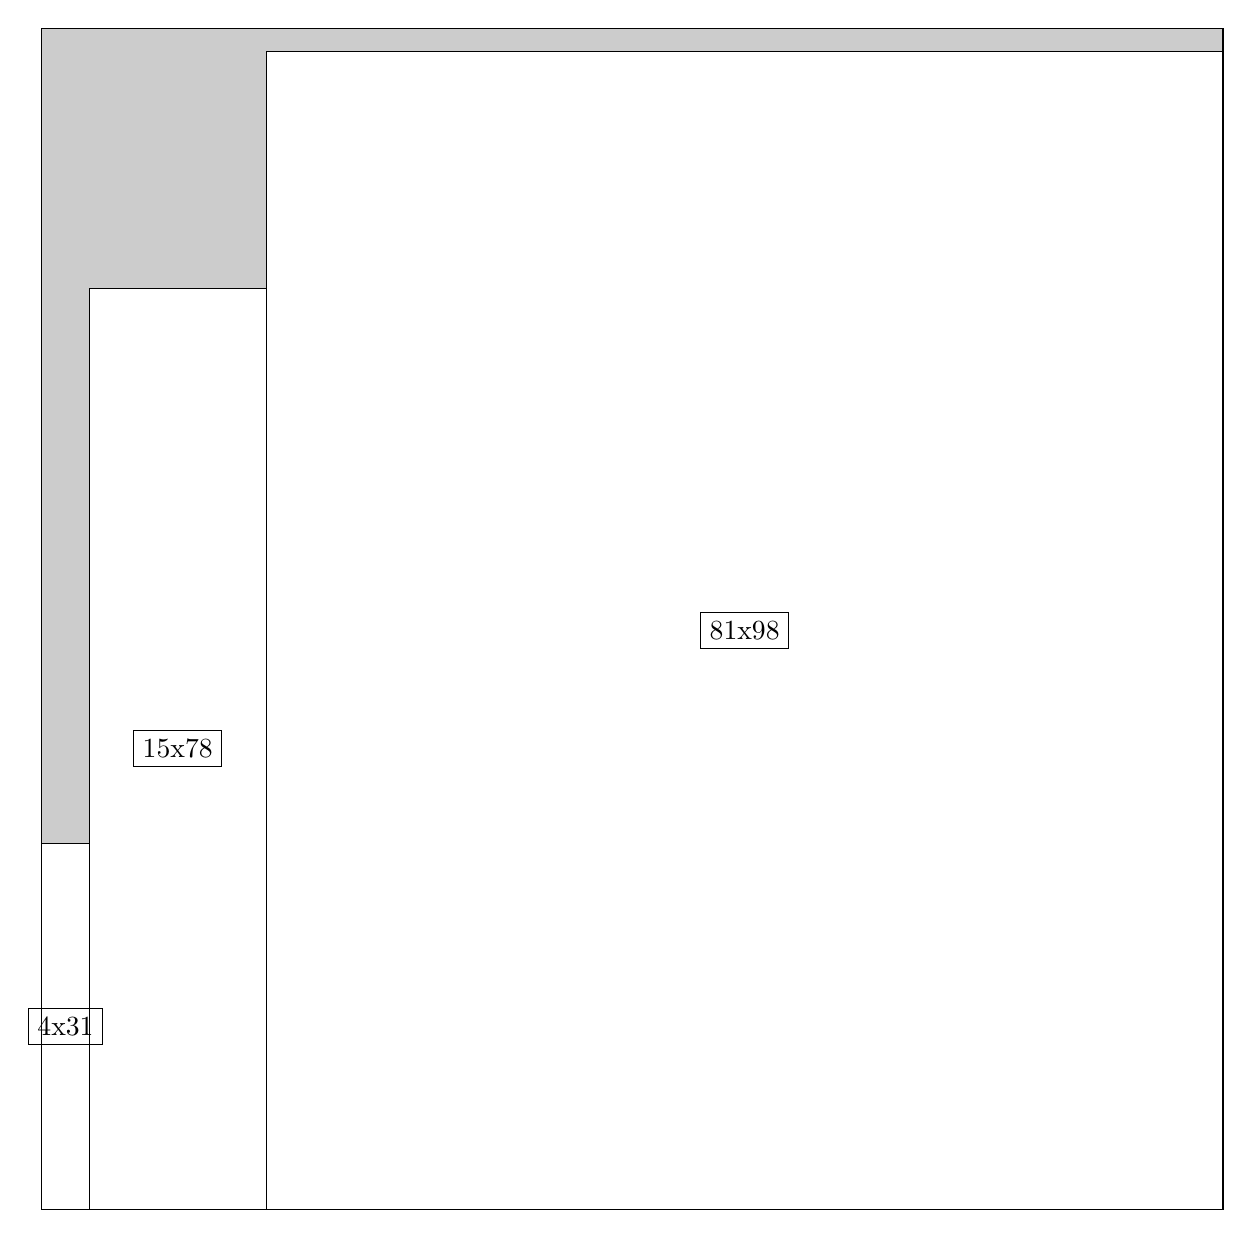
\begin{tikzpicture}[shorten >=1pt,scale=1.0,every node/.style={scale=1.0},->]
\tikzstyle{vertex}=[circle,fill=black!25,minimum size=14pt,inner sep=0pt]
\filldraw[fill=gray!40!white, draw=black] (0,0) rectangle (15.0,15.0);
\foreach \name/\x/\y/\w/\h in {81x98/2.85/0.0/12.15/14.7,15x78/0.6/0.0/2.25/11.7,4x31/0.0/0.0/0.6/4.6499999999999995}
\filldraw[fill=white!40!white, draw=black] (\x,\y) rectangle node[draw] (\name) {\name} ++(\w,\h);
\end{tikzpicture}


w =81 , h =98 , x =19 , y =0 , v =7938
\par
w =15 , h =78 , x =4 , y =0 , v =1170
\par
w =4 , h =31 , x =0 , y =0 , v =124
\par
\newpage


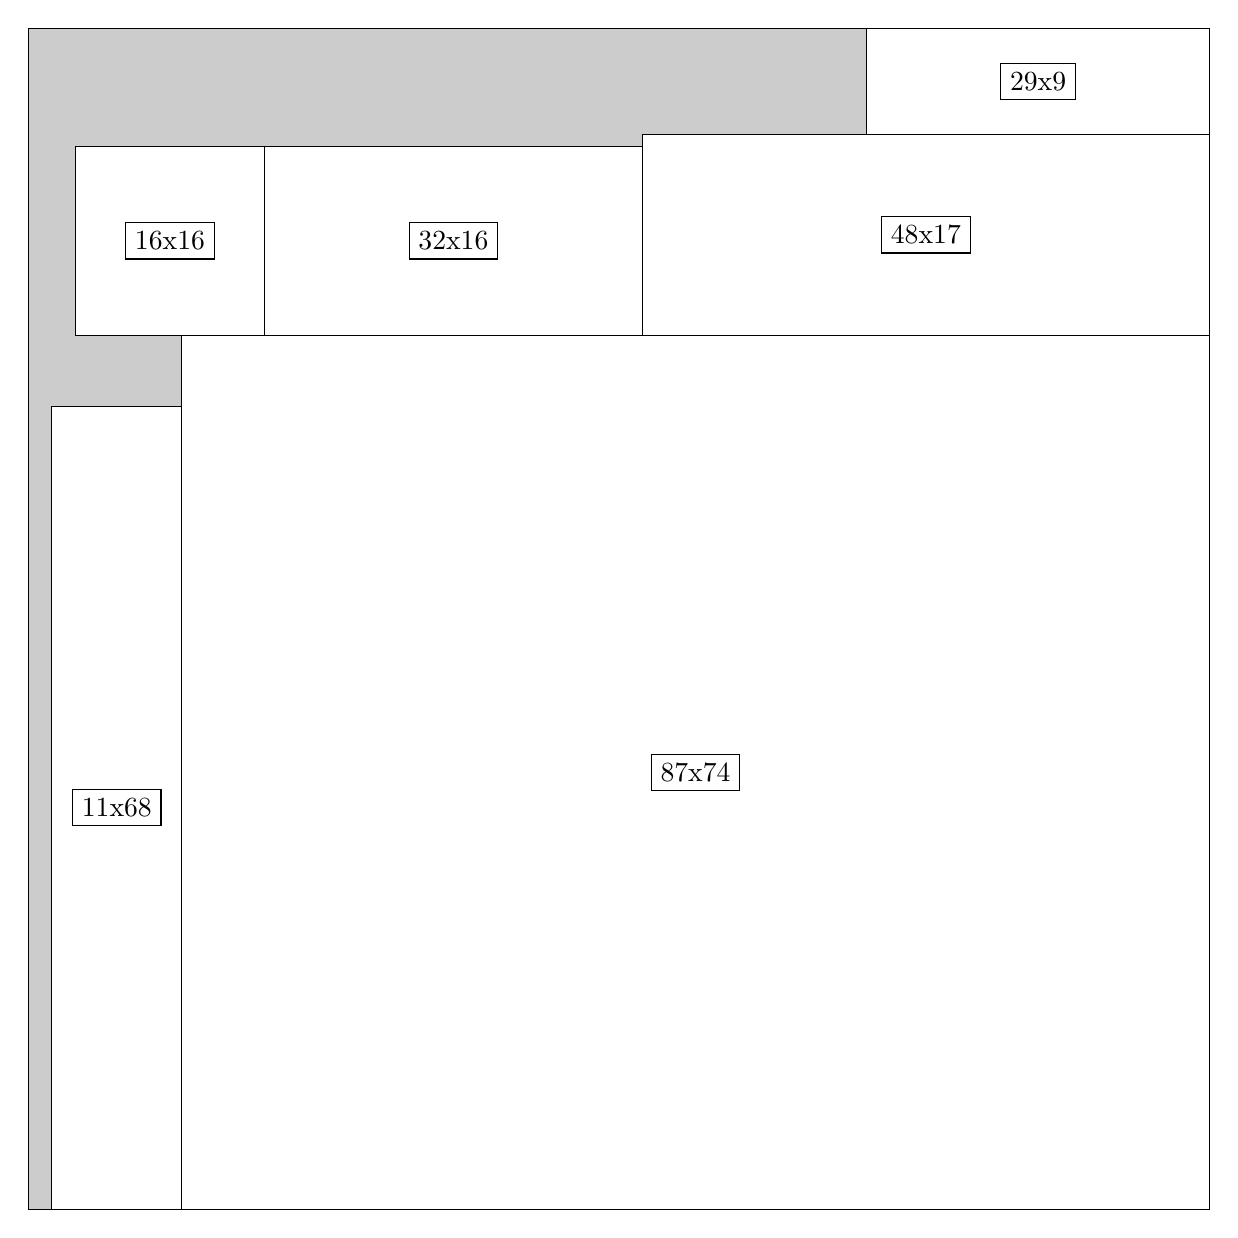
\begin{tikzpicture}[shorten >=1pt,scale=1.0,every node/.style={scale=1.0},->]
\tikzstyle{vertex}=[circle,fill=black!25,minimum size=14pt,inner sep=0pt]
\filldraw[fill=gray!40!white, draw=black] (0,0) rectangle (15.0,15.0);
\foreach \name/\x/\y/\w/\h in {87x74/1.95/0.0/13.049999999999999/11.1,11x68/0.3/0.0/1.65/10.2,48x17/7.8/11.1/7.199999999999999/2.55,29x9/10.65/13.65/4.35/1.3499999999999999,32x16/3.0/11.1/4.8/2.4,16x16/0.6/11.1/2.4/2.4}
\filldraw[fill=white!40!white, draw=black] (\x,\y) rectangle node[draw] (\name) {\name} ++(\w,\h);
\end{tikzpicture}


w =87 , h =74 , x =13 , y =0 , v =6438
\par
w =11 , h =68 , x =2 , y =0 , v =748
\par
w =48 , h =17 , x =52 , y =74 , v =816
\par
w =29 , h =9 , x =71 , y =91 , v =261
\par
w =32 , h =16 , x =20 , y =74 , v =512
\par
w =16 , h =16 , x =4 , y =74 , v =256
\par
\newpage


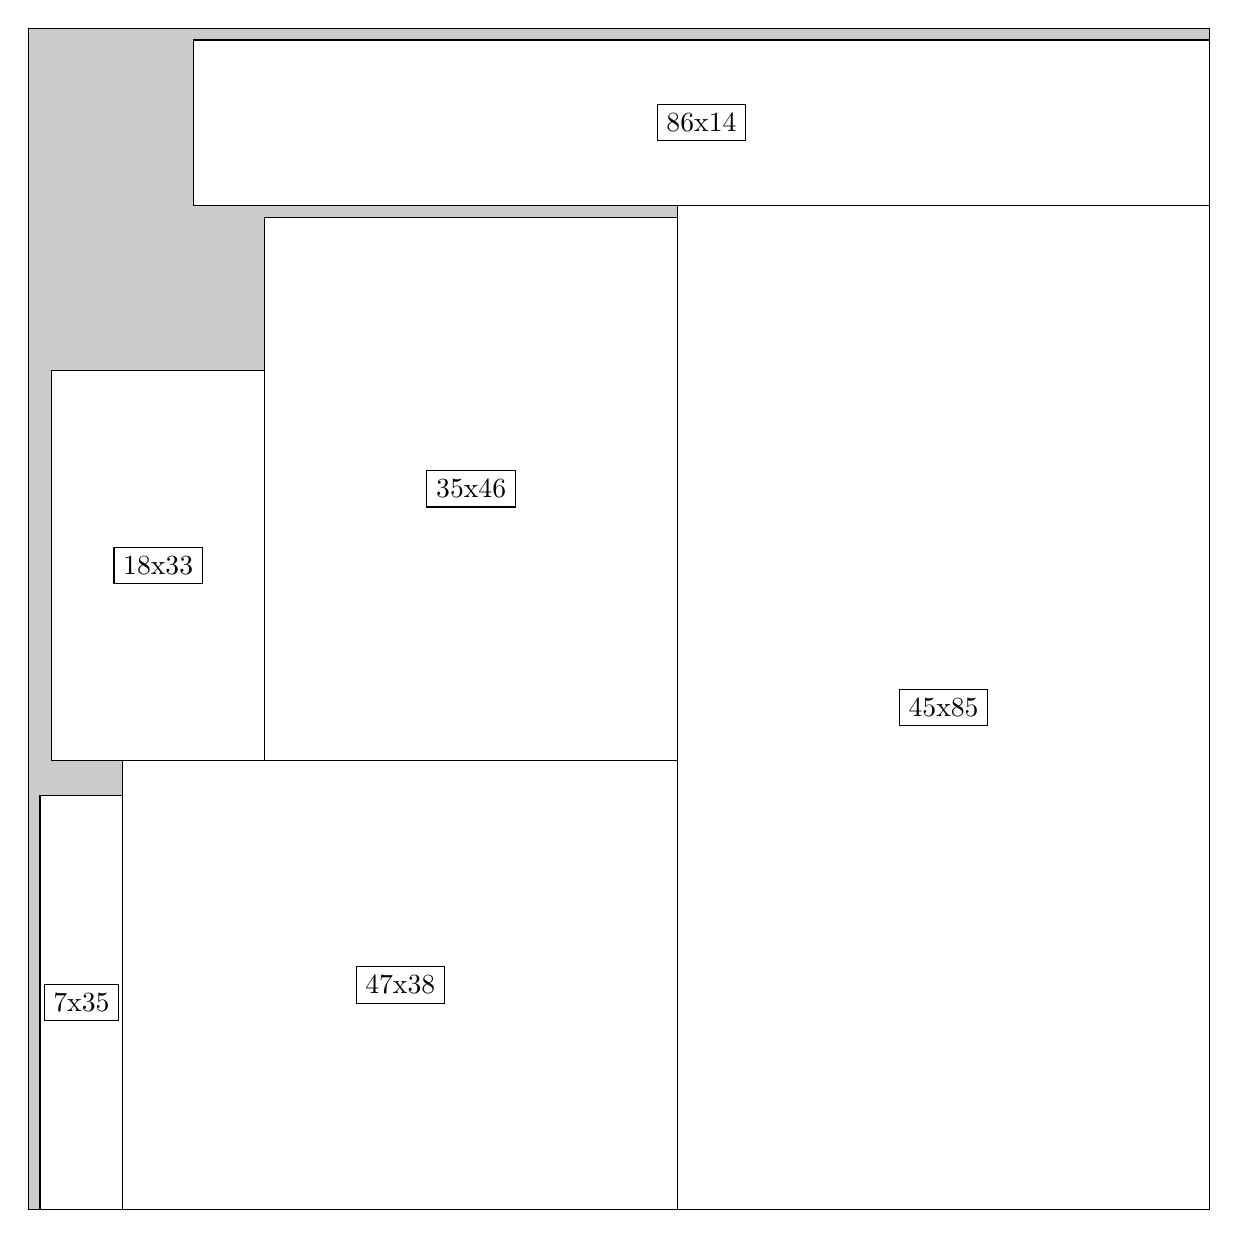
\begin{tikzpicture}[shorten >=1pt,scale=1.0,every node/.style={scale=1.0},->]
\tikzstyle{vertex}=[circle,fill=black!25,minimum size=14pt,inner sep=0pt]
\filldraw[fill=gray!40!white, draw=black] (0,0) rectangle (15.0,15.0);
\foreach \name/\x/\y/\w/\h in {45x85/8.25/0.0/6.75/12.75,47x38/1.2/0.0/7.05/5.7,7x35/0.15/0.0/1.05/5.25,35x46/3.0/5.7/5.25/6.8999999999999995,18x33/0.3/5.7/2.6999999999999997/4.95,86x14/2.1/12.75/12.9/2.1}
\filldraw[fill=white!40!white, draw=black] (\x,\y) rectangle node[draw] (\name) {\name} ++(\w,\h);
\end{tikzpicture}


w =45 , h =85 , x =55 , y =0 , v =3825
\par
w =47 , h =38 , x =8 , y =0 , v =1786
\par
w =7 , h =35 , x =1 , y =0 , v =245
\par
w =35 , h =46 , x =20 , y =38 , v =1610
\par
w =18 , h =33 , x =2 , y =38 , v =594
\par
w =86 , h =14 , x =14 , y =85 , v =1204
\par
\newpage


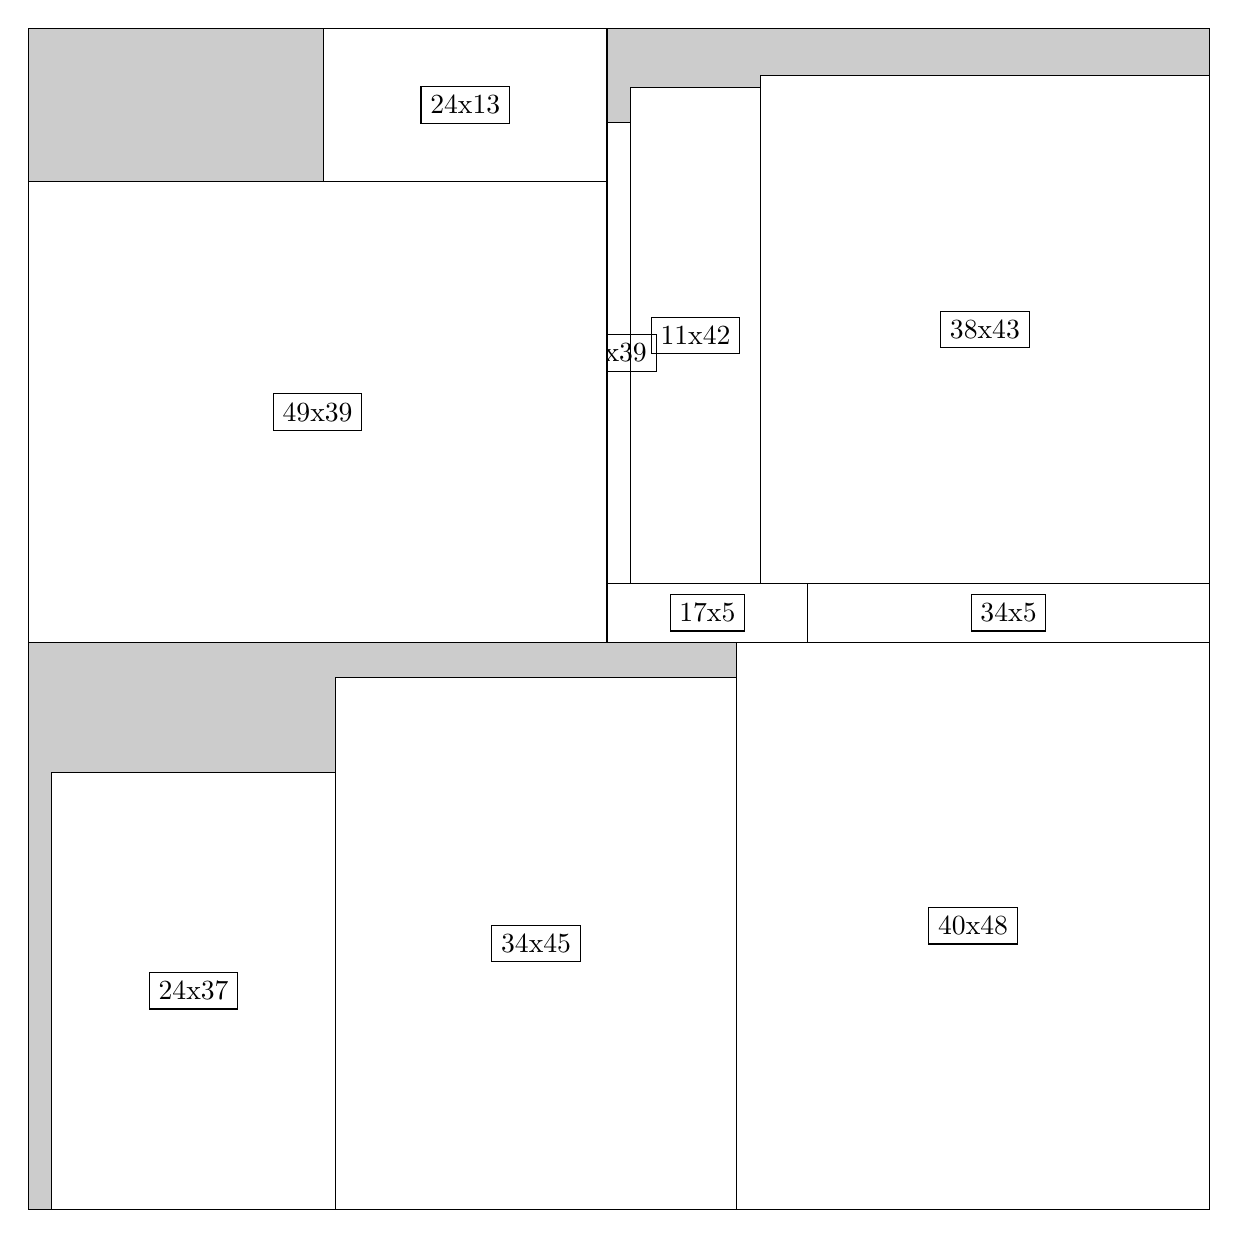
\begin{tikzpicture}[shorten >=1pt,scale=1.0,every node/.style={scale=1.0},->]
\tikzstyle{vertex}=[circle,fill=black!25,minimum size=14pt,inner sep=0pt]
\filldraw[fill=gray!40!white, draw=black] (0,0) rectangle (15.0,15.0);
\foreach \name/\x/\y/\w/\h in {40x48/9.0/0.0/6.0/7.199999999999999,34x45/3.9/0.0/5.1/6.75,24x37/0.3/0.0/3.5999999999999996/5.55,34x5/9.9/7.199999999999999/5.1/0.75,17x5/7.35/7.199999999999999/2.55/0.75,38x43/9.299999999999999/7.949999999999999/5.7/6.45,11x42/7.6499999999999995/7.949999999999999/1.65/6.3,2x39/7.35/7.949999999999999/0.3/5.85,49x39/0.0/7.199999999999999/7.35/5.85,24x13/3.75/13.049999999999999/3.5999999999999996/1.95}
\filldraw[fill=white!40!white, draw=black] (\x,\y) rectangle node[draw] (\name) {\name} ++(\w,\h);
\end{tikzpicture}


w =40 , h =48 , x =60 , y =0 , v =1920
\par
w =34 , h =45 , x =26 , y =0 , v =1530
\par
w =24 , h =37 , x =2 , y =0 , v =888
\par
w =34 , h =5 , x =66 , y =48 , v =170
\par
w =17 , h =5 , x =49 , y =48 , v =85
\par
w =38 , h =43 , x =62 , y =53 , v =1634
\par
w =11 , h =42 , x =51 , y =53 , v =462
\par
w =2 , h =39 , x =49 , y =53 , v =78
\par
w =49 , h =39 , x =0 , y =48 , v =1911
\par
w =24 , h =13 , x =25 , y =87 , v =312
\par
\newpage


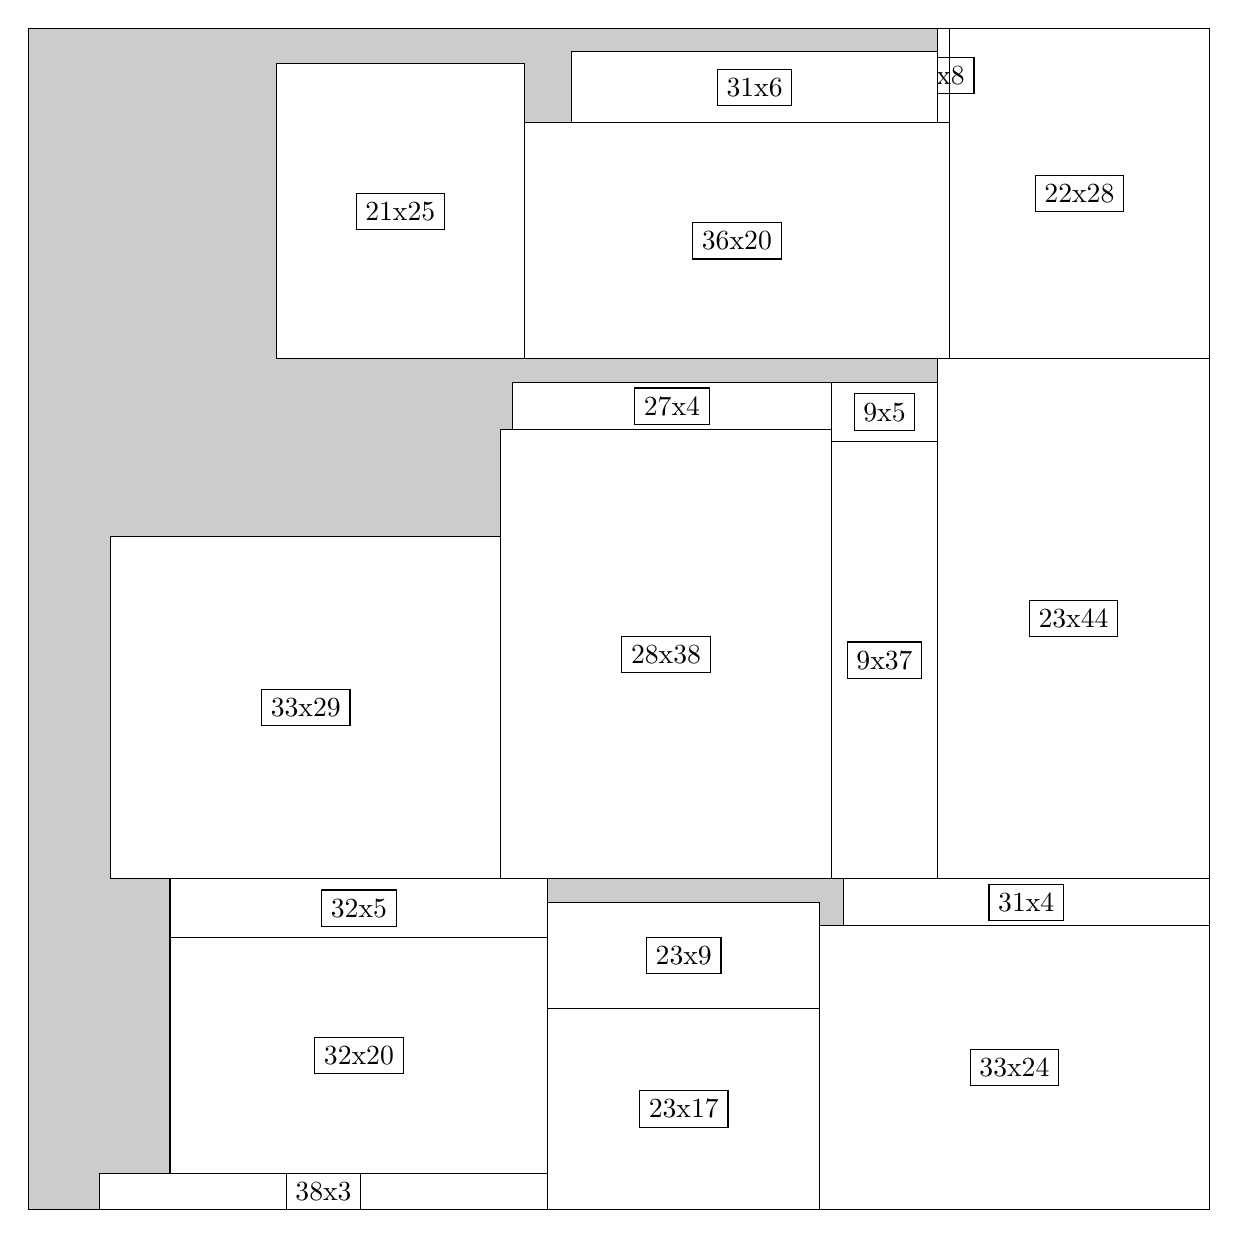
\begin{tikzpicture}[shorten >=1pt,scale=1.0,every node/.style={scale=1.0},->]
\tikzstyle{vertex}=[circle,fill=black!25,minimum size=14pt,inner sep=0pt]
\filldraw[fill=gray!40!white, draw=black] (0,0) rectangle (15.0,15.0);
\foreach \name/\x/\y/\w/\h in {33x24/10.049999999999999/0.0/4.95/3.5999999999999996,31x4/10.35/3.5999999999999996/4.6499999999999995/0.6,23x17/6.6/0.0/3.4499999999999997/2.55,23x9/6.6/2.55/3.4499999999999997/1.3499999999999999,38x3/0.8999999999999999/0.0/5.7/0.44999999999999996,32x20/1.7999999999999998/0.44999999999999996/4.8/3.0,32x5/1.7999999999999998/3.4499999999999997/4.8/0.75,23x44/11.549999999999999/4.2/3.4499999999999997/6.6,9x37/10.2/4.2/1.3499999999999999/5.55,9x5/10.2/9.75/1.3499999999999999/0.75,28x38/6.0/4.2/4.2/5.7,27x4/6.1499999999999995/9.9/4.05/0.6,33x29/1.05/4.2/4.95/4.35,22x28/11.7/10.799999999999999/3.3/4.2,36x20/6.3/10.799999999999999/5.3999999999999995/3.0,1x8/11.549999999999999/13.799999999999999/0.15/1.2,31x6/6.8999999999999995/13.799999999999999/4.6499999999999995/0.8999999999999999,21x25/3.15/10.799999999999999/3.15/3.75}
\filldraw[fill=white!40!white, draw=black] (\x,\y) rectangle node[draw] (\name) {\name} ++(\w,\h);
\end{tikzpicture}


w =33 , h =24 , x =67 , y =0 , v =792
\par
w =31 , h =4 , x =69 , y =24 , v =124
\par
w =23 , h =17 , x =44 , y =0 , v =391
\par
w =23 , h =9 , x =44 , y =17 , v =207
\par
w =38 , h =3 , x =6 , y =0 , v =114
\par
w =32 , h =20 , x =12 , y =3 , v =640
\par
w =32 , h =5 , x =12 , y =23 , v =160
\par
w =23 , h =44 , x =77 , y =28 , v =1012
\par
w =9 , h =37 , x =68 , y =28 , v =333
\par
w =9 , h =5 , x =68 , y =65 , v =45
\par
w =28 , h =38 , x =40 , y =28 , v =1064
\par
w =27 , h =4 , x =41 , y =66 , v =108
\par
w =33 , h =29 , x =7 , y =28 , v =957
\par
w =22 , h =28 , x =78 , y =72 , v =616
\par
w =36 , h =20 , x =42 , y =72 , v =720
\par
w =1 , h =8 , x =77 , y =92 , v =8
\par
w =31 , h =6 , x =46 , y =92 , v =186
\par
w =21 , h =25 , x =21 , y =72 , v =525
\par
\newpage


\end{document}